%&latex

\documentclass{article}
\usepackage{amsmath}
\usepackage{graphicx}


\DeclareMathOperator*{\argmax}{argmax}

\begin{document}

%+Title
\title{Interactive Video Lecture Summary}
\author{Hijung V.Shin}
\date{\today}
\maketitle
%-Title

%+Abstract
%\begin{abstract}
%    There is abstract text that you should replace with your own. 
%\end{abstract}
%-Abstract

%+Contents
%\tableofcontents
%-Contents

\section{Segmentation}

\subsection{Line break algorithm}
\subsection{Energy function}
In summary, the score for a set of lines is the sum of the following terms (multiplied by constant coefficients and raised to constant powers):
\begin{itemize}
\item{sum of the number of horizontally aligned strokes in each line}
\item{sum of number of strokes in each line}
\item{weighted average of the compactness of each line}
\item{negative of the maximum horizontal gap in each line (xgap)}
\item{negative of the maximum vertical gap in each line}
\item{negative of the overlapping area between lines}
\end{itemize}

\begin{figure}[!h]
\center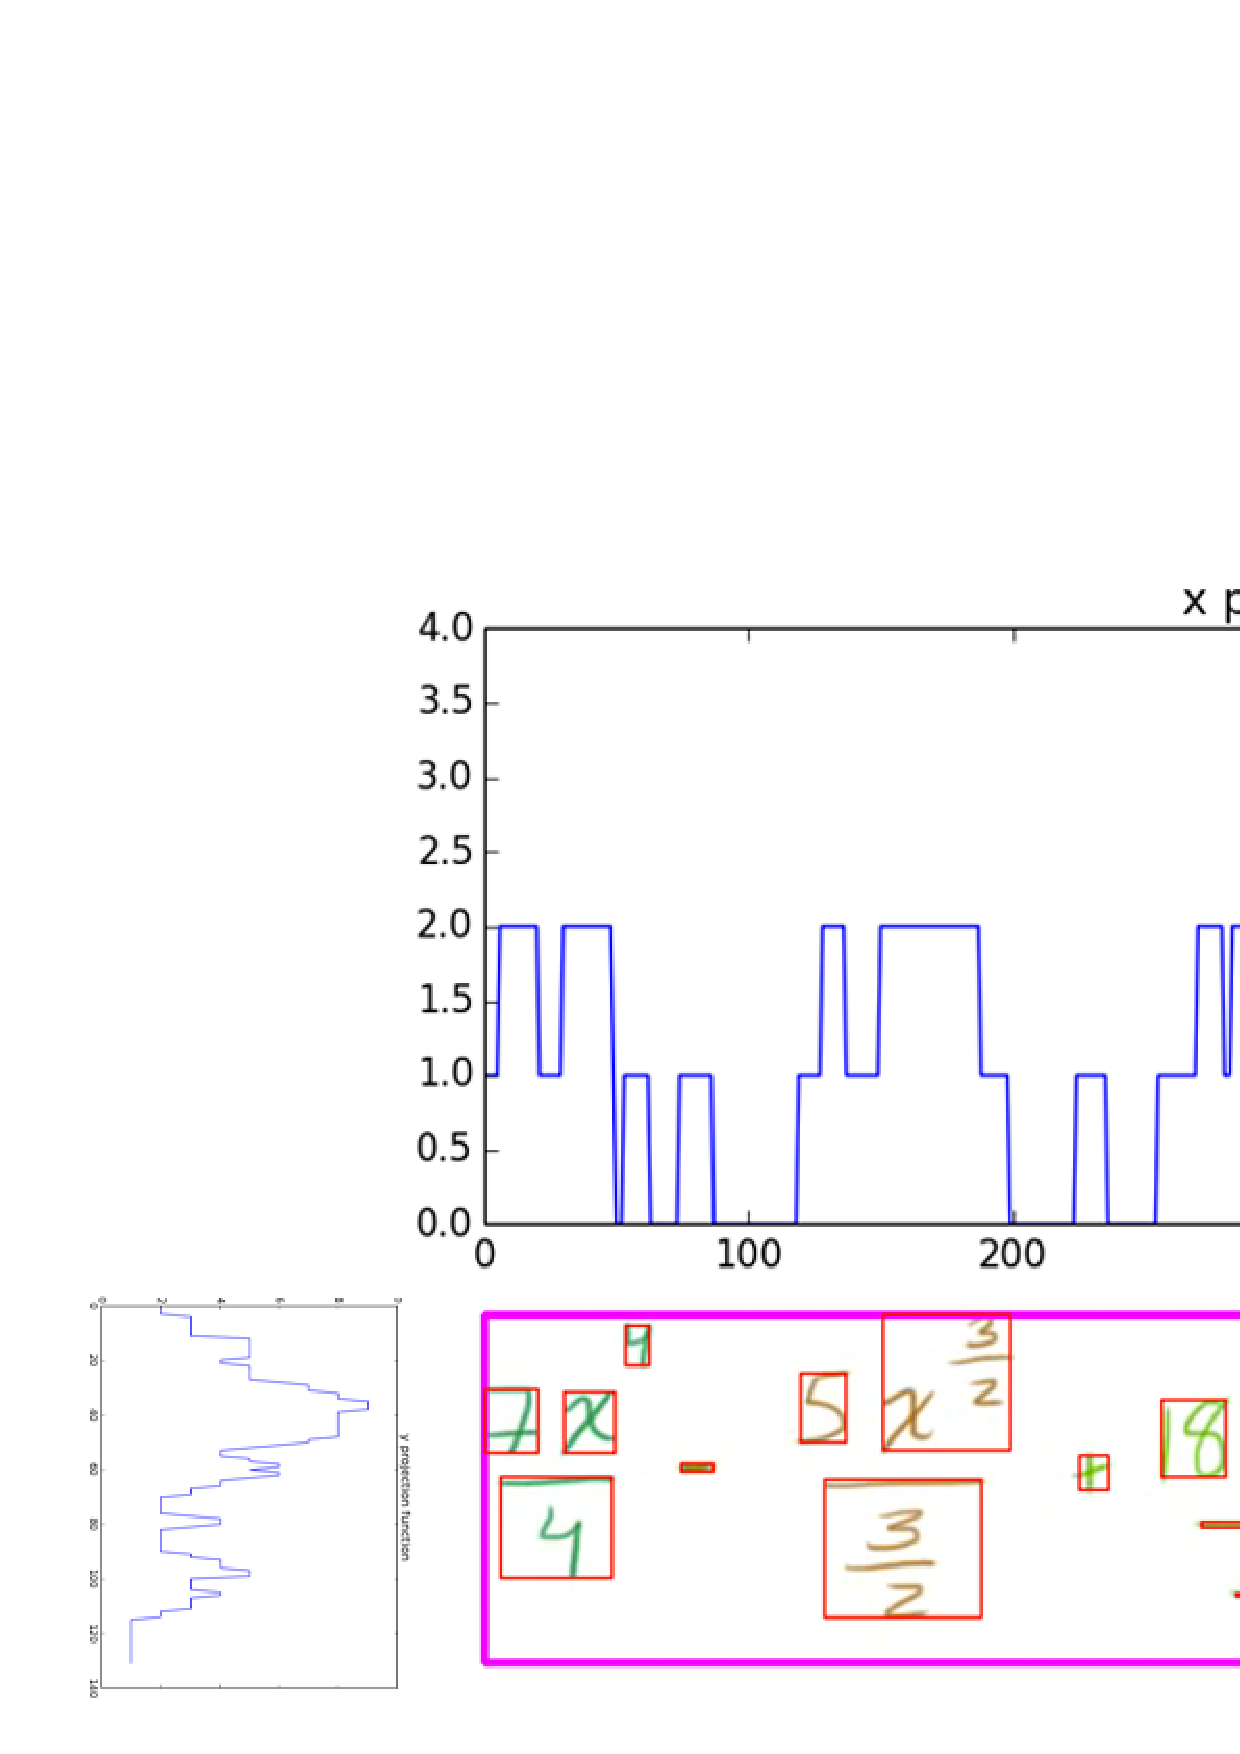
\includegraphics[width=\textwidth]{figures/proj_function_example}

\end{figure}
\begin{figure}[!h]
\center
\end{figure}

More formally, consider $C_s$ the set of all strokes drawn during a lecture. Our goal is to segment the strokes into mutually exclusive lines or figures, $C_{s_1}, C_{s_2}, ...$ such that 
\begin{align}
\bigcup \limits_{i} C_i = C_s\\
C_i \cap C_j = \emptyset\quad \forall i \ne j
\end{align} \\
To this purpose we define a scoring function which, given a set of sets of strokes $C_{s_i}$'s returns a scalar value indicating the \textit{badness} of the segmentation. The scoring function depends on several factors.
\\
\begin{enumerate}
\item The number of strokes in each line:
 
\begin{equation}
n_\text{strokes}(C_{s_i}) = \big{|}C_{s_i}\big{|}
\end{equation}\\
\item The number of horizontally aligned strokes in each line: In order to identify strokes that are aligned horizontally, we define a \textit{horizontal projection function}, $proj_h$, as\\
\begin{equation}
proj_h(y, C_{s_i}) = \big{|}\{s\in C_{s_i} \small{|} y_\text{min}(s)\le y \le y_{max}(s) \}\big{|}
\end{equation}\\
where $y_\text{min}(s)$ and $y_\text{max}(s)$ return the minimum and maximum y coordinate of the bounding box for stroke $s$. \\
Then given a candidate line $C_{s_i}$, the maximum number of horizontally aligned strokes, $n_\text{aligned}(C_{s_i})$, is defined as
\begin{equation}
n_\text{aligned}(C_{s_i}) = \argmax_{y_\text{min}(C_{s_i}) \le y \le y_\text{max}(C_{s_i})} f(y)
\end{equation}\\
\item
The maximum horizontal gap in a line. $x_\text{gap}(C_{s_i})$, is defined using the \textit{vertical projection function}
\begin{equation}
proj_v(x, C_{s_i}) = \big|\{s \in C_{s_i} \small| x_\text{min}(s) \le x \le x_\text{max}(s)\}\big|
\end{equation}
\begin{equation}
x_\text{gap}(C_{s_i}) = \argmax_{x_i, x_{i+1} \in proj_{v:C_{s_i} \ne 0}} (x_{i+1} - x_i)
\end{equation}
where $proj_{v:C_{s_i} \ne 0}$ is an ordered set such that $x_{i} \in proj_{v:C_{s_i}}$ if $proj_v(x_{i}, C_{s_i}) \ne 0$, and $x_i \le x_{i+1}$.\\
\item
Similarly, we can define the maximum vertical gap in a line, $y_\text{gap}(C_{s_i})$.
\item The compactness of a line, measured as:
\begin{equation}
comp(C_{s_i}) = \frac{\sum\limits_{s\in C_s}area(s)}{area(C_{s_i})}
\end{equation}
where $area(s)$ is the area of the bounding box of stroke $s$.
\item Finally, given a set of lines $L$, the overlap penalty, $P_{overlap}$, is defined as
\begin{equation}
P_{overlap}(L) = \sum \limits_{C_{s_i}, C_{s_j} \in L} \frac{area(overlap(C_{s_i}, C_{s_j}))}{min(area(C_{s_i}), area(C_{s_j}))}
\end{equation}
\end{enumerate}
The score of a segmentation $L$ is defined as:
\begin{align}
score(L) &=\sum\limits_{C_{s_i}\in L}\Bigg{(}n_\text{aligned}(C_{s_i})^{\alpha_{1}}+n_\text{strokes}(C_{s_i})^{\alpha_{2}}\Bigg{)}\\ &-\sum\limit_{C_{s_i}\in L}\Bigg{(}x_\text{gap}(C_{s_i})^{\alpha_3}+y_\text{gap}(C_{s_i})^{\alpha_4}\Bigg{)}\\
&+\frac{\sum\limits_{C_{s_i} \in L} (npix(C_{s_i})\times comp(C_{s_i}))}{\sum\limits_{C_{s_i} \in L}npix(C_{s_i})}\\
&- P_{overlap}(L)
\end{align}


%+Bibliography
\begin{thebibliography}{}
\bibitem{}
\end{thebibliography}
%-Bibliography

\end{document}



